\documentclass[10pt,aspectratio=169]{beamer}

% All the boilerplate is in deslides.sty
\usepackage{deslides}

\author{Ji\v{r}\'i Lebl}

\institute[OSU]{%
Oklahoma State University%
%Departemento pri Matematiko de Oklahoma {\^S}tata Universitato%
}

\title{11. Exact equations\\(Notes on Diffy Qs, 1.8)}

\date{}

\begin{document}

\begin{frame}
\titlepage

%\bigskip

\begin{center}
The textbook: \url{https://www.jirka.org/diffyqs/}
\end{center}
\end{frame}

\begin{frame}
An \emph{exact equation} is an equation that encodes 
\[
F(x,y) = \text{constant}
\]
for a \emph{potential function} $F(x,y)$.

\medskip
\pause

Naming suggests electric potential or potential energy.

\medskip
\pause

Such equations come up when there is some conservation
law (e.g., conservation of energy) at play.

\end{frame}

\begin{frame}
\textbf{Example:}
Let $F(x,y) = x^2+y^2$

%16 is the number of lines, must be adjusted
\vspace*{-\baselineskip}
\hspace*{3in}%
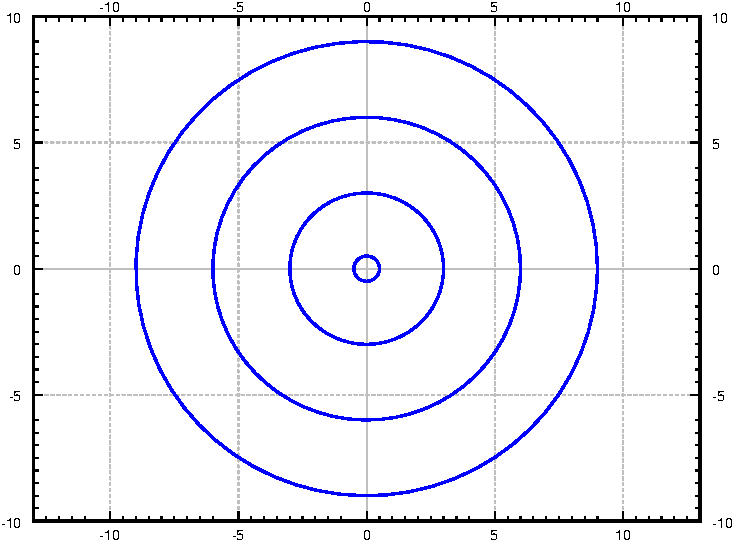
\includegraphics[width=2.5in]{../figures/circlesfig}

\hspace*{3in}%
Solutions to $F(x,y) = x^2+y^2 = C$.

\vspace*{-1.8in}

\pause

Take the
\emph{total derivative} of
$F$:

\medskip
\quad
$dF =
\dfrac{\partial F}{\partial x} dx + \dfrac{\partial F}{\partial y} dy
=
F_x dx + F_y dy
$.

\medskip
\pause
So
$dF = 2x \, dx + 2y \, dy$.

\medskip
\pause

To get $F(x,y) = C$, the differential equation is

\medskip

\quad $dF = 0$.

\medskip
\pause

In this case,

\medskip

\quad
$2x \, dx + 2y \, dy = 0$
\quad
or
\quad
$2x + 2y \, \dfrac{dy}{dx} = 0$
\end{frame}

\begin{frame}

In general, \quad
$M \, dx + N \, dy = 0$, \quad
or
\quad
$M + N \, \frac{dy}{dx} = 0$ \quad
is exact if it is \quad $dF = 0$.

\medskip
\pause

In other words, $M \, dx + N \, dy = 0$ is exact if there is an $F$ such that $M = F_x$ and $N=F_y$.

\medskip
\pause

So 
\quad
$2x \, dx + 2y \, dy = 0$
\quad
is exact.

\medskip
\pause

$x^2+y^2=C$ are implicit solutions.

\medskip
\pause

$y = \pm \sqrt{C^2-x^2}$ are the explicit solutions.

\medskip
\pause

Normally, we start with $M \, dx + N \, dy = 0$ and we wish to find the
unknown $F(x,y)$.
\end{frame}

\begin{frame}
\textbf{Interpretation:}
At each point $(x,y)$, the vector $\vec{v} = (M,N)$ gives a \emph{vector
field}.

\medskip
\pause

$\vec{v}$ is a \emph{conservative vector field} if it comes with a potential
function $F$ where
$\vec{v} = \left( \frac{\partial F}{\partial x} ,\frac{\partial F}{\partial
y} \right)$.

\medskip
\pause

Let $\gamma$ be a path in the plane from $(x_1,y_1)$ and ending at
$(x_2,y_2)$ and think of $\vec{v}$ as force.

\medskip

The work required to move along $\gamma$ is
\quad
$\displaystyle
\int_\gamma \vec{v}(\vec{r}) \cdot d\vec{r}
=
\int_\gamma M \, dx + N \, dy
=
F(x_2,y_2) - F(x_1,y_1)$.

\medskip
\pause

In other words, work done depends only on endpoints.

\medskip
\pause

\textbf{Example:} Force of gravity $\vec{v}$ is conservative (assuming 2D),
and $F$ is the gravitational potential.
\pause
Work done by moving a mass only depends on the change in elevation.

\medskip
\pause

Exact equations are conservative vector fields, and
their
implicit solutions are given by the potential functions.

\end{frame}

\begin{frame}
The process is, we are given
an equation
\quad
$M + N \, \frac{dy}{dx} = 0$

\medskip
\pause

We need to then determine if the equation is exact.

\medskip
\pause

If it is, we need to find an $F$ such that $F_x = M$
and $F_y = N$.

\medskip
\pause

$F\bigl(x,y(x)\bigr) = C$ gives an implicit solution

\medskip
\pause

Note that adding a constant to $F$ does not change anything.

\pause
If $F(x,y)$ works, $F(x,y)+3$ or $F(x,y)-8$ also work.

\end{frame}

\begin{frame}

\textbf{Example:}
Consider \quad $2x + 2y \frac{dy}{dx} = 0$. \quad  Forget we knew
what $F$ was.

\medskip
\pause

$M = 2x$ and $N=2y$.

\medskip
\pause

If $F$ exists, $F_x (x,y) = 2x$.

\medskip
\pause

Integrate in $x$:
\quad
$F(x,y) = x^2 + A(y)$,
\quad
for some function $A(y)$ (constant of integration).

\medskip
\pause

Differentiate in $y$ and set it equal to $N$:

\medskip
\quad
$2y = F_y (x,y) = A'(y)$.

\medskip
\pause

Integrate $2y=A'(y)$: \quad
$A(y) = y^2$ \quad (no need for a constant of integration).

\medskip
\pause

So

\medskip

\quad
$F(x,y) = x^2 + A(y) = x^2+y^2$.

\end{frame}

\begin{frame}

The procedure (if equation is exact):
\begin{enumerate}[(i)]
\item
\pause
Integrate $F_x = M$ in $x$ resulting in $F(x,y) = \text{something} + A(y)$.
\item
\pause
Differentiate $F$ in $y$, and set that equal to
$N$ to find $A(y)$ by integration.
\end{enumerate}
\pause
Roles of $x$ and $y$ can be reversed.

\end{frame}

\begin{frame}

\textbf{Example:}
Consider now $2x+y + xy \frac{dy}{dx} = 0$.

\medskip
\pause

$M = 2x+y$, \quad $N=xy$.

\medskip
\pause

We try as before.  Suppose $F$ exists.

\medskip
\pause

$F_x (x,y) = 2x+y$.

\medskip
\pause

Integrate in $x$: \quad $F(x,y) = x^2 + xy + A(y)$

\medskip
\pause

Differentiate in $y$ and set equal to $N$:

\medskip
\pause

$N = xy = F_y (x,y) = x+A'(y)$.

\medskip
\pause

But there is no way to write $xy = x+ A'(y)$, no matter what $A'(y)$ is.

\medskip
\pause

The equation is not exact!  $F$ does not exist.
\end{frame}

\begin{frame}
How to check if $F$ exists?

\medskip
\pause

If $F$ exists, then
$M = F_x$ and
$N = F_y$.

\medskip
\pause

Then
\[
\frac{\partial M}{\partial y}
\pause
=
\frac{\partial^2 F}{\partial y \partial x}
\pause
=
\frac{\partial^2 F}{\partial x \partial y}
\pause
=
\frac{\partial N}{\partial x} .
\]
\pause
In other words:

\begin{theorem}[Poincar\'e]
If $M$ and $N$ are continuously differentiable functions of $(x,y)$, and
$\frac{\partial M}{\partial y} = \frac{\partial N}{\partial x}$,
then near any point there is a function $F(x,y)$
such that
$M = \frac{\partial F}{\partial x}$ and
$N = \frac{\partial F}{\partial y}$.
\end{theorem}

\pause

\textbf{Note:} The theorem doesn't say a \emph{global} $F$ exists, only \emph{local}.

\medskip
\pause

Back to example: If $M = 2x + y$ and $N = xy$,  
then
$M_y = 1$ and  $N_x = y$.
\pause
Not equal.
\pause
Not exact.

\end{frame}

\begin{frame}

\textbf{Example:}
Solve
\begin{equation*}
\frac{dy}{dx} = \frac{-2x-y}{x-1}, \qquad y(0) = 1.
\end{equation*}
We write the equation as
\begin{equation*}
(2x+y) + (x-1)\frac{dy}{dx} = 0 ,
\end{equation*}
so $M = 2x+y$ and $N = x-1$.  Then
\begin{equation*}
M_y = 1 = N_x .
\end{equation*}
The equation is exact.
Integrating $M$ in $x$, we find
\begin{equation*}
F(x,y) = x^2+xy + A(y) .
\end{equation*}
Differentiating in $y$ and setting to $N$, we find
\begin{equation*}
x-1 = x + A'(y) .
\end{equation*}
So $A'(y) = -1$, and $A(y) = -y$ will work.  Take $F(x,y) = x^2+xy-y$.  We
wish to solve $x^2+xy-y = C$.  First let us find $C$.  As $y(0)=1$ then
$F(0,1) = C$.  Therefore $0^2+0\times 1 - 1 = C$, so $C=-1$.  Now we solve
$x^2+xy-y = -1$ for $y$ to get
\begin{equation*}
y = \frac{-x^2-1}{x-1} .
\end{equation*}
\end{frame}

\begin{frame}

\textbf{Example:}
Solve
\begin{equation*}
-\frac{y}{x^2+y^2} dx + \frac{x}{x^2+y^2} dy = 0 , \qquad y(1) = 2.
\end{equation*}
We leave to the reader to check that
$M_y = N_x$.

This vector field $(M,N)$ is not conservative if considered as a vector
field of the entire plane minus the origin.  The problem is that if the curve $\gamma$
is a circle around the origin, say starting at $(1,0)$ and
ending at $(1,0)$ going counterclockwise, then if $F$ existed we would expect
\begin{equation*}
0 = F(1,0) - F(1,0) = \int_\gamma F_x \, dx + F_y \, dy = \int_\gamma \frac{-y}{x^2+y^2} \, dx +
\frac{x}{x^2+y^2} \, dy = 2\pi .
\end{equation*}
That is nonsense!
We leave the computation of the path integral to the interested reader, or
you can consult your multivariable calculus textbook.  So there is no
potential function $F$ defined everywhere outside the origin $(0,0)$.

If we think back to the theorem, it does not guarantee such a function
anyway.  It only guarantees a potential function locally, that is, only in
some region near the initial point.  As $y(1) = 2$,
we start at the point $(1,2)$.  Considering $x > 0$ and
integrating $M$ in $x$ or $N$ in $y$, we find
\begin{equation*}
F(x,y) = \operatorname{arctan} \bigl( \nicefrac{y}{x} \bigr) .
\end{equation*}
The implicit solution is 
$\operatorname{arctan} \bigl( \nicefrac{y}{x} \bigr) = C$.  Solving,
$y = \tan(C) x$.  That is, the solution is a straight line.  Solving $y(1) =
2$ gives us that $\tan(C) = 2$, and so $y= 2x$ is the desired solution.
See {exact:y2x}, and note that the solution only exists for $x >
0$.

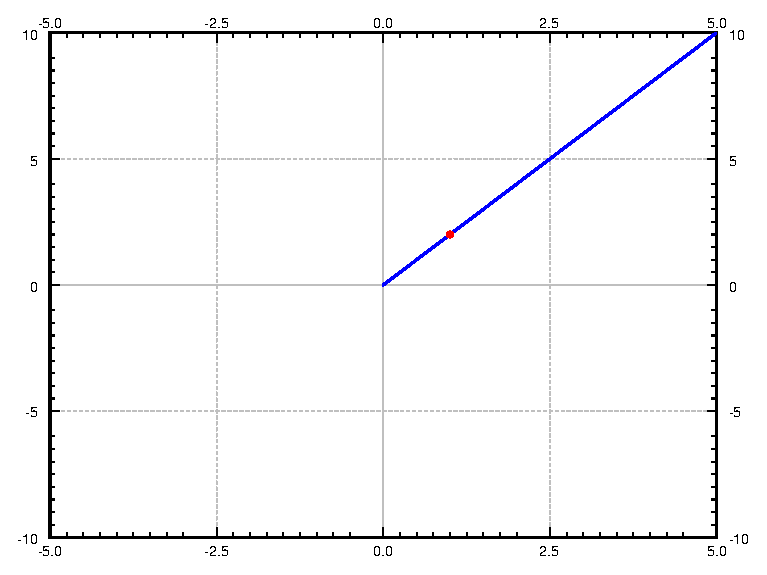
\includegraphics[width=2.5in]{../figures/exact-y2x}

Solution to 
$-\frac{y}{x^2+y^2} dx + \frac{x}{x^2+y^2} dy = 0$, $y(1) = 2$,
with initial point marked.
\end{frame}

\begin{frame}

\textbf{Example:}
Solve
\begin{equation*}
x^2+y^2 + 2y(x+1) \frac{dy}{dx} = 0 .
\end{equation*}

The reader should check that this equation is exact.
Let $M= x^2+y^2$ and $N=2y(x+1)$.
We follow the procedure for exact equations
\begin{equation*}
F(x,y) = \frac{1}{3}x^3 + xy^2 + A(y) ,
\end{equation*}
and
\begin{equation*}
2y(x+1) = 2xy + A'(y) .
\end{equation*}
Therefore $A'(y) = 2y$ or $A(y) = y^2$ and $F(x,y) = \frac{1}{3}x^3 + xy^2 +
y^2$.
We try to solve $F(x,y) = C$.  We easily solve for $y^2$ and then just take
the square root:
\begin{equation*}
y^2 = \frac{C-(\nicefrac{1}{3})x^3}{x+1},
\qquad \text{so} \qquad
y = \pm \sqrt{\frac{C-(\nicefrac{1}{3})x^3}{x+1}} .
\end{equation*}
When $x=-1$, the term in front of $\frac{dy}{dx}$ vanishes, and our explicit
solution is not valid at $x=-1$.
The given equation has no solution near $x=-1$, but
the equation $(x^2+y^2) \, dx + 2y(x+1) \, dy = 0$ does have
a solution $x=-1$.  In fact, one could solve for $x$ in terms
of $y$ for any initial condition.  The solution is messy,
so we leave it as $\frac{1}{3}x^3 + xy^2 + y^2 = C$.
\end{frame}

\begin{frame}

{Integrating factors}

Sometimes an equation $M\, dx + N \, dy = 0$ is not exact, but it can be
made exact by multiplying with a function $u(x,y)$.  That is, perhaps
for some nonzero function $u(x,y)$,
\begin{equation*}
u(x,y) M(x,y) \, dx + u(x,y) N(x,y) \, dy = 0
\end{equation*}
is exact.  Any solution to this new equation is also a solution to
$M\, dx + N \, dy = 0$.

In fact, a linear equation
\begin{equation*}
\frac{dy}{dx} + p(x) y = f(x), \qquad
\text{or} \qquad
\bigl( p(x) y - f(x) \bigr)\, dx +  dy  = 0
\end{equation*}
is always such an equation.  Let $r(x) = e^{\int p(x)\,dx}$ be the
integrating factor for a linear equation.  Multiply the equation by $r(x)$
and write it in the form of $M + N \frac{dy}{dx} = 0$.
\begin{equation*}
r(x) p(x) y - r(x) f(x) + r(x) \frac{dy}{dx} = 0 .
\end{equation*}
Then $M = r(x) p(x) y - r(x) f(x)$, so
$M_y = r(x) p(x)$, while $N = r(x)$, so
$N_x = r'(x) = r(x) p(x)$.  In other words, we have an exact equation.
Integrating
factors for linear functions are just a special case of integrating
factors for exact equations.

But how do we find the integrating factor $u$?  Well, given an equation
\begin{equation*}
M \, dx + N \, dy = 0 ,
\end{equation*}
$u$ should be a
function such that
\begin{equation*}
\frac{\partial}{\partial y} \bigl[ u M \bigr] = 
u_y M + u M_y = 
\frac{\partial}{\partial x} \bigl[ u N \bigr] = 
u_x N + u N_x .
\end{equation*}
Therefore,
\begin{equation*}
(M_y-N_x)u = u_x N - u_y M .
\end{equation*}
At first it may seem we replaced one differential equation by another.
True, but all hope is not lost.

A strategy that often works is to look for a $u$ that is a function
of $x$ alone, or a function of $y$ alone.  If $u$ is a function of $x$
alone,
that is $u(x)$, then we write $u'(x)$ instead of $u_x$, and $u_y$ is just
zero.
Then
\begin{equation*}
\frac{M_y-N_x}{N}u = u' .
\end{equation*}
In particular, $\frac{M_y-N_x}{N}$ ought to be a function of $x$ alone (not
depend on $y$).  If so, then we have a linear equation
\begin{equation*}
u' - \frac{M_y-N_x}{N} u = 0 .
\end{equation*}
Letting $P(x) = \frac{M_y-N_x}{N}$,
we solve using the standard integrating factor method,
to find $u(x) = C e^{\int P(x) \, dx}$.  The constant in the
solution is not relevant, we need any nonzero solution,
so we take $C=1$.
Then $u(x) = e^{\int P(x) \, dx}$ is the integrating factor.

Similarly, we could try a function of the form $u(y)$.
Then
\begin{equation*}
\frac{M_y-N_x}{M} u = - u' .
\end{equation*}
In particular, $\frac{M_y-N_x}{M}$ ought to be a function of $y$ alone.
If so, we have a linear equation
\begin{equation*}
u' + \frac{M_y-N_x}{M} u = 0 .
\end{equation*}
Letting $Q(y) = \frac{M_y-N_x}{M}$,
we find $u(y) = C e^{-\int Q(y) \, dy}$.  We
take $C=1$.  So $u(y) = e^{-\int Q(y) \, dy}$ is the integrating factor.

\end{frame}

\begin{frame}

\textbf{Example:}
Solve
\begin{equation*}
\frac{x^2+y^2}{x+1} + 2y \frac{dy}{dx} = 0 .
\end{equation*}

Let $M= \frac{x^2+y^2}{x+1}$ and $N=2y$.
Compute
\begin{equation*}
M_y-N_x = \frac{2y}{x+1} - 0 = \frac{2y}{x+1} .
\end{equation*}
As this is not zero, the equation is not exact.  We notice 
\begin{equation*}
P(x) = \frac{M_y-N_x}{N} = \frac{2y}{x+1} \, \frac{1}{2y} = \frac{1}{x+1} 
\end{equation*}
is a function of $x$ alone.    We compute the integrating factor
\begin{equation*}
e^{\int  P(x) \, dx}
=
e^{\ln (x+1)} = x+1 .
\end{equation*}
We multiply our given equation by $(x+1)$ to obtain
\begin{equation*}
x^2+y^2 + 2y(x+1) \frac{dy}{dx} = 0 ,
\end{equation*}
which is an exact equation that we solved in
{exact:exampleabove}.  The solution was
\begin{equation*}
y = \pm \sqrt{\frac{C-(\nicefrac{1}{3})x^3}{x+1}} .
\end{equation*}
\end{frame}

\begin{frame}
\textbf{Example:}
Solve
\begin{equation*}
y^2 + (xy+1) \frac{dy}{dx} = 0 .
\end{equation*}

First compute
\begin{equation*}
M_y-N_x = 2y-y = y .
\end{equation*}
As this is not zero, the equation is not exact.  We observe
\begin{equation*}
Q(y) = \frac{M_y-N_x}{M} = \frac{y}{y^2} = \frac{1}{y} 
\end{equation*}
is a function of $y$ alone.    We compute the integrating factor
\begin{equation*}
e^{-\int  Q(y) \, dy}
=
e^{-\ln y} = \frac{1}{y} .
\end{equation*}
Therefore, we look at the exact equation
\begin{equation*}
y + \frac{xy+1}{y} \frac{dy}{dx} = 0 .
\end{equation*}
The reader should double check that this equation is exact.
We follow the procedure for exact equations
\begin{equation*}
F(x,y) = xy + A(y) ,
\end{equation*}
and
\begin{equation}
\frac{xy+1}{y} = x+\frac{1}{y} = x+ A'(y) .
\end{equation}
Consequently, $A'(y) = \nicefrac{1}{y}$ or $A(y) = \ln \, \lvert y \rvert$.  Thus $F(x,y)
= xy + \ln \, \lvert y \rvert$.
It is not possible to solve $F(x,y)=C$ for $y$
in terms of elementary functions, so 
let us be content with the implicit solution:
\begin{equation*}
xy + \ln \, \lvert y \rvert = C .
\end{equation*}
We are looking for the general solution and we divided by
$y$ above.  We should check what happens when $y=0$, as the equation itself
makes perfect sense in that case.  We plug in $y=0$ to find the
equation is satisfied.  So $y=0$ is also a solution.
\end{frame}

\end{document}
